\documentclass[tikz,border=6pt]{standalone}
\usepackage{xcolor}
\usetikzlibrary{arrows.meta,positioning}

\definecolor{blockblue}{HTML}{4A90D9}
\definecolor{linegray}{HTML}{333333}

\begin{document}
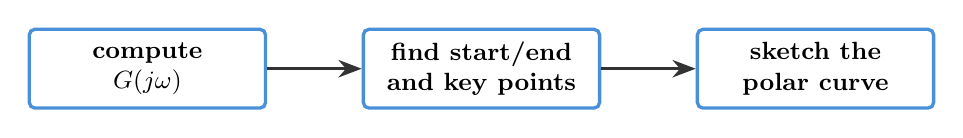
\begin{tikzpicture}[
  >=Stealth,
  line width=1.2pt,
  stage/.style={rectangle, draw=blockblue, rounded corners=2pt, minimum width=3.0cm, minimum height=1.0cm, align=center, font=\small\bfseries},
  flow/.style={->, draw=linegray, line width=1.2pt}
]
  \node[stage] (s1) at (0,0) {compute\\$G(j\omega)$};
  \node[stage, right=1.2cm of s1] (s2) {find start/end\\and key points};
  \node[stage, right=1.2cm of s2] (s3) {sketch the\\polar curve};
  \draw[flow] (s1) -- (s2);
  \draw[flow] (s2) -- (s3);
\end{tikzpicture}
\end{document}
